% ============================================================================
%  Chapitre 5, partie VI : Campagne de Monte-Carlo
% ============================================================================

% ----------------------------------------------------------------------------
\section{Campagne de Monte-Carlo}
% ----------------------------------------------------------------------------

La partie précédente montre que notre estimation fonctionne sur les deux cas. On
veut maintenant savoir à quel point elle fonctionne en général, en la
lançant sur un grand nombre de scénarios tirés au hasard.

\subsection{Tirage des paramètres}

Un scénario est décrit par la variable aléatoire
\[
    X = (\vect{q}_0, \vect{\Omega}_0, m, a, \mat{I}_b, \mat{P})
\]
dont les composantes sont tirées indépendamment :
\begin{itemize}
    \item l'orientation initiale $\vect{q}_0$ et le montage $\mat{P}$
    sont uniformes sur $\SO$, tirés à partir d'un quaternion unitaire
    uniforme, plutôt que sur les intervalles qui définissent les angles d'Euler 
    pour éviter la concentration près des pôles. (Imaginons que l'on soit dans le cas d'un globle
    avec la longitude et la latitude, les lignes se concentrent aux pôles).
    \item $\vect{\Omega}_0$, $m$ et $a$ sont uniformes sur les
    intervalles du tableau~\ref{tab-lois-mc}.
    \item $\mat{I}_b = ma^2\,\mathrm{diag}(\lambda_1, \lambda_2, \lambda_3)$,
    où les moments propres $\lambda_i$ sont uniformes sur
    $[\lambda_{\min}, \lambda_{\max}]$.
\end{itemize}

Le gyromètre garde les réglages de la partie V : $f = 100$~Hz,
$\sigma = 5\cdot 10^{-3}$~rad/s, biais selon $\mathcal{N}(0, 10^{-6}\Id)$,
et $5$~s de mesure. Certes, dans la réalité, le biais a des drifts, et la fréquence de capteur n'est pas tout le temps $100\%$ à cause des bruits ou de mauvais timing dans le code. Pour ce niveau de validation, je le garderai pour la validation finale.

\begin{table}[H]
    \centering
    \begin{tabular}{lcc}
        \toprule
        Paramètre & Loi & Intervalle \\
        \midrule
        $\vect{q}_0$, $\mat{P}$ & uniforme sur $\SO$ & \\
        $\Omega_{0,x}$, $\Omega_{0,y}$ (rad/s) & uniforme & $[-2;\ 2]$ \\
        $\Omega_{0,z}$ (rad/s) & uniforme & $[-6;\ 6]$ \\
        $m$ (kg) & uniforme & $[0{,}5;\ 2]$ \\
        $a$ (m) & uniforme & $[0{,}05;\ 0{,}15]$ \\
        $\lambda_1, \lambda_2, \lambda_3$ & uniforme & $[0{,}1;\ 1]$ \\
        \bottomrule
    \end{tabular}
    \caption{Lois des paramètres de la campagne de Monte-Carlo}
    \label{tab-lois-mc}
\end{table}
\textbf{Validation du scénario : } le résultat d'un scénario n'est gardé que s'il est
physique et exploitable :
\begin{itemize}
    \item inégalités d'inertie : $\lambda_1 + \lambda_2 \ge \lambda_3$ (et
    permutations).

    \item masse dans la boule : $\lambda_1 + \lambda_2 + \lambda_3 \le 2$,
    car $I_1 + I_2 + I_3 = 2\int \|\vect{x}\|^2\,\mathrm{d}m \le 2ma^2$.
    \item mouvement assez excité : $\|\vect{\Omega}_0\| \ge \Omega_{\min}$,
    sinon rien ne se passera.
    \item non-glissement vérifié sur toute la simulation : $|N| \le \mu_s m g$.
\end{itemize}
Sinon, on retire le scénario. $X$ suit donc la loi uniforme conditionnée
à l'ensemble des scénarios admissibles.

\subsection{Critères et Estimation de la Performance de la méthode}

\textbf{Erreur relative de moment d'inertie d'un scénario : } pour le scénario $X_k$, la simulation
donne la vraie matrice $\mat{J}_k = \mat{P}_k\mat{I}_{b,k}\mat{P}_k^T$, et
l'estimation donne $\hat{\mat{J}}_k$. On définit l'erreur relative d'inertie
\[
    \varepsilon_k = \frac{\|\hat{\mat{J}}_k - \mat{J}_k\|_F}{\|\mat{J}_k\|_F}
\]

\textbf{Variable de succès de la méthode pour un scénario : } pour une tolérance $\mathrm{tol_{est}}$ fixée,
on pose
\[
    S_k = \mathbf{1}_{\{\varepsilon_k < \mathrm{tol_{est}}\}}
\]
Les scénarios sont indépendants et de même loi, donc les $S_k$ sont des
variables de Bernoulli indépendantes de paramètre
\[
    p = \mathbb{P}(\varepsilon < \mathrm{tol_{est}}) = \mathbb{E}[S_k]
\]
le taux de réussite de la méthode, ce qui décrit la performance. Le nombre de succès sur $N$
scénarios suit alors la loi binomiale $\mathcal{B}(N, p)$.

\textbf{Estimation de $p$ : } on estime $p$ par la proportion de
succès
\[
    \hat{p}_N = \frac{1}{N}\sum_{k=1}^{N} S_k
\]
qui est sans biais, $\mathbb{E}[\hat{p}_N] = p$, de variance
$p(1-p)/N$, et qui converge presque sûrement vers $p$ par la LFGN. Par le théorème central limite, un intervalle de
confiance à $95\,\%$ est
\[
    \hat{p}_N \pm 1{,}96\sqrt{\frac{\hat{p}_N(1-\hat{p}_N)}{N}}
\]
\subsection{Résultat}

On lance la campagne sur $N = 3000$ scénarios admissibles. Aucune
estimation n'échoue, et $\mat{\Phi}^T\mat{\Phi}$ est toujours inversible.

\begin{figure}[H]
    \centering
    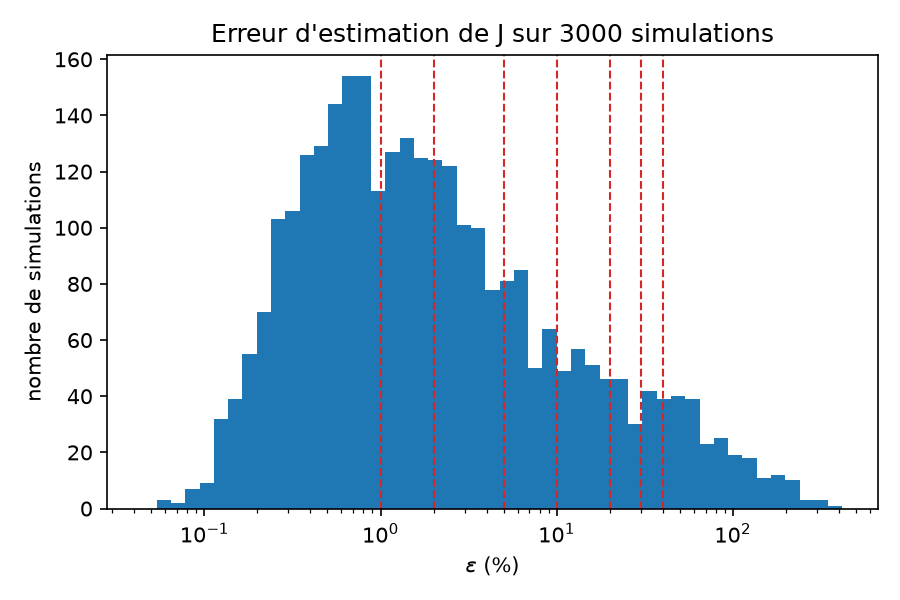
\includegraphics[width=0.75\textwidth]{chapitre5/figures/hist_eps.png}
    \caption{Distribution de l'erreur $\varepsilon$ sur les $3000$
    scénarios (échelle logarithmique), les pointillés sont les
    tolérances du tableau~\ref{tab-taux-mc}}
    \label{fig-hist-eps}
\end{figure}
\begin{figure}[H]
    \centering
    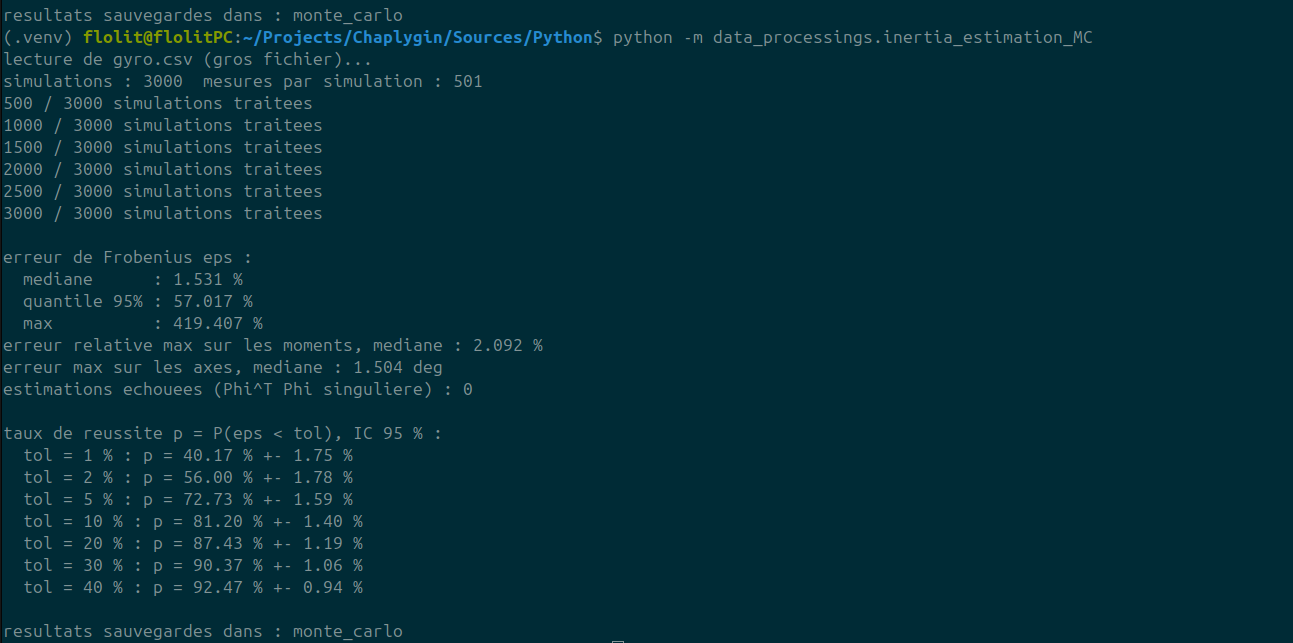
\includegraphics[width=0.75\textwidth]{chapitre5/figures/Result_3000sims.png}
    \caption{Résultats des $3000$ simulations}
    \label{fig-terminal}
\end{figure}
\newpage
Voici le résultat du traitement de données de la simulation Monte-Carlo.
\begin{table}[H]
    \centering
    \begin{tabular}{cc}
        \toprule
        $\mathrm{tol_{est}}$ & $\hat{p}_N$ (IC $95\,\%$) \\
        \midrule
        $1\,\%$  & $40{,}2 \pm 1{,}8\,\%$ \\
        $2\,\%$  & $56{,}0 \pm 1{,}8\,\%$ \\
        $5\,\%$  & $72{,}7 \pm 1{,}6\,\%$ \\
        $10\,\%$ & $81{,}2 \pm 1{,}4\,\%$ \\
        $20\,\%$ & $87{,}4 \pm 1{,}2\,\%$ \\
        $30\,\%$ & $90{,}4 \pm 1{,}1\,\%$ \\
        $40\,\%$ & $92{,}5 \pm 0{,}9\,\%$ \\
        \bottomrule
    \end{tabular}
    \caption{Taux de réussite estimé selon la tolérance}
    \label{tab-taux-mc}
\end{table}

\textbf{Commentaires : }
\begin{itemize}
    \item Pour un scénario typique, la méthode marche bien : l'erreur
    médiane est près de $\varepsilon = 1{,}5\,\%$.
    \item La distribution a pourtant une longue queue : $\approx 10\,\%$ des
    scénarios ont une erreur au-delà de $30\,\%$.
\end{itemize}
\begin{proposition}[Ce qu'il faudra faire]
    Jusqu'à ce stade, l'idée de l'algorithme est validée, on a une estimation suffisamment satisfaisante. Afin d'avoir une meilleure performance, il nous faut alors étudier les grosses erreurs et leurs causes.
\end{proposition}

